Considera los dos triángulos que se muestran abajo en la figura \ref{fig:20230323155215} (los triángulos no están dibujados a escala).

\begin{minipage}{0.6\textwidth}
    \textbf{¿Los dos triángulos son congruentes?}\\
    \emph{Escoge 1 respuesta y explica el por qué:}\\

    \begin{choices}
        \CorrectChoice Sí.
        \choice No.
        \choice No hay suficiente información para decidir.
    \end{choices}
    \vspace{2cm}
\end{minipage}%
\begin{minipage}{0.35\textwidth}
    \begin{figure}[H]
        \centering
        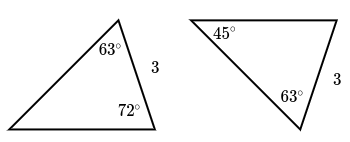
\includegraphics[width=\linewidth]{../images/20230323155215}
        \caption{}
        \label{fig:20230323155215}
    \end{figure}
\end{minipage}

\begin{solutionbox}{5cm}\footnotesize
    \begin{minipage}{0.65\textwidth}
        Dos triángulos son congruentes si tienen la misma forma y tamaño. En otras palabras, dos triángulos son congruentes si todos los lados y ángulos correspondientes son congruentes.
        Sin embargo, no necesitamos mostrar la congruencia de todos los lados y ángulos correspondientes para demostrar que dos triángulos son congruentes. Los criterios de congruencia (LLL, LAL, ALA) y el teorema AAL son atajos útiles para determinar congruencia de triángulos.
        En este caso, nos dan un lado y dos ángulos en cada triángulo.
        Puesto que la suma de las medidas de los ángulos de un triángulo es 180$^\circ$, podemos encontrar el ángulo restante en cada triángulo.
        Ahora observa que dos ángulos y el lado entre ellos en un triángulo son congruentes a dos ángulos y el lado entre ellos de otro triángulo.
        Por lo tanto, los triángulos son congruentes por el criterio ALA.
        \textbf{Sí, los triángulos son congruentes.}
    \end{minipage}\hfill
    \begin{minipage}{0.25\textwidth}
        \begin{figure}[H]
            \centering
            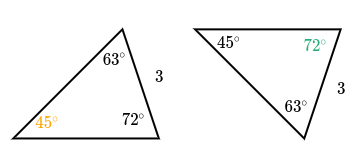
\includegraphics[width=\linewidth]{../images/20230323155725}
            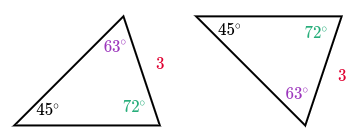
\includegraphics[width=\linewidth]{../images/20230323155732}
            \caption{}
            \label{fig:20230323155725}
        \end{figure}

        % \begin{figure}[H]
        %     \centering
        %     \caption{}
        %     \label{fig:20230323155732}
        % \end{figure}
    \end{minipage}
\end{solutionbox}